% O treinamento de uma rede neural de convolução~\footnote{\url{http://caffe.berkeleyvision.org/}} foi realizado, utilizando as classes ``praia'' e ``montanha'', balanceadas, da base Corel-1000. A classificação sobre este treinamento obteve $\approx 80\%$ de acurácia, enquanto que utilizando os extratores padrões foi possível atingir apenas $\approx 69\%$. Isso reforça a proposta de analisar quais são as características latentes que esse tipo de rede neural consegue extrair. Para essa análise vão ser utilizadas bases discriminadas quanto às propriedades de textura, cor e forma.

São muitos os aspectos que influenciam a classificação de imagens. É comum lidar com as particularidades das características extraídas ao invés de se preocupar com o tratamento das imagens no início do \textit{pipeline}. Portanto, o enfoque desta pesquisa foi na investigação de métodos de processamento de imagens antes da extração de características. Para tal, esta dissertação propôs duas abordagens para melhorar a discriminação entre classes: realizar a quantização com o objetivo de obter vetores de características mais compactos; e gerar imagens artificiais a partir das imagens originais de forma a rebalancear a base de imagens.

Os resultados encontrados ao usar os métodos de quantização de imagens apontam para uma alternativa --- ou complemento --- à seleção de características. Dado o número de cores limitado na imagem original, a quantidade de possíveis características a serem extraídas é reduzida, especialmente as de cor. A extração de características de textura também é facilitada, considerando que normalmente é computada utilizando uma memória proporcional ao número de intensidades.

Ficou constatado que um vetor original de $D$ dimensões pode ser reduzido a $d \approx D/4$ modificando apenas o parâmetro de quantização e produzindo resultados significativos. Ou seja, de 256 intensidades para apenas 64. Outra possibilidade é utilizar esses métodos como um primeiro passo de redução e então utilizar o LPP para obter apenas 100 características que melhor representam os dados, atingindo acurácias maiores ou similares.

É importante ressaltar que realizar a quantização de imagens não requer treinamento e já faz parte de uma tarefa do próprio \textit{pipeline} de reconhecimento. Por esta razão, seu uso não aumenta o custo computacional do sistema, e ainda simplifica os passos subsequentes. Isso reduz a dimensão do vetor de características para os vetores de cor e o tempo de computação para os descritores de textura. Outra observação importante é que a quantização é usada especialmente para dados visuais, então não é um método geral de redução de dimensionalidade.

Além disso, com os experimentos realizados foi possível notar que a geração de imagens artificiais pode gerar novas informações para a classificação das imagens. Assim, a geração de elementos no espaço visual contribuiu com o balanceamento entre classes, melhorando a acurácia de algoritmos de classificação, inclusive quando comparada à geração de exemplos artificiais no espaço de atributos (i.e.\ SMOTE). Para validar a proposta da geração artificial de imagens, uma visualização do espaço de características foi realizada. As características das novas imagens e os exemplos resultantes da interpolação de vetores originais foram projetados no plano das imagens originais antes do desbalanceamento. Dessa forma foi possível visualizar que a geração de imagens artificiais proposta foi capaz de ocupar uma região do espaço mais abrangente do que o SMOTE. Este último possui o ponto negativo de não extrapolar os limites da classe minoritária. Ainda, está suscetível à criação de novos exemplos em regiões da classe majoritária, o que também prejudica a classificação.

\section{Publicações}

Foi publicado um artigo na revista \textit{Neurocomputing}, referente aos resultados de quantização desta pesquisa \cite{Ponti2016}. O artigo referente à geração de imagens artificiais para o rebalanceamento de classes está em preparo.

% \begin{figure}[hbpt]
%  \begin{center}
%    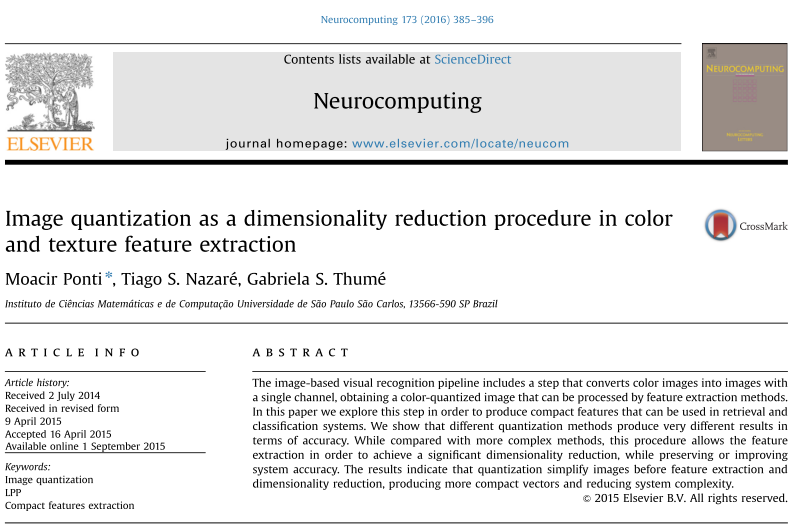
\includegraphics[width=\linewidth]{figuras/artigo.png}
%  \end{center}
%  \caption{Artigo publicado na \textit{Neurocomputing}, referente a quantização de imagens. \textit{Fonte~\url{http://www.sciencedirect.com/science/article/pii/S0925231215012771}}.}
%  \label{fig:artigo}
% \end{figure}

\section{Trabalhos Futuros}

% Ao utilizar imagens com reduzido número de intensidades (quantizadas), os métodos de extração de características baseados em orientação (HoG, SIFT), \textit{bag of visual words} e \textit{Fisher vectors}, seriam provavelmente mais esparsos. Portanto, estudos futuros da influência da quantização em outros métodos de extração de características podem ser realizados.

Visto que o método MSB se sobressaiu nos resultados do uso da quantização, variações desse método podem produzir melhores mapas de cor para a etapa de reconhecimento. A investigação dos espaços gerados por tais métodos também pode fornecer uma melhor análise da discriminação entre classes.

Estudos futuros da influência da quantização em outros métodos de extração de características podem ser realizados. Por exemplo, ao utilizar imagens com reduzido número de intensidades (quantizadas), métodos de extração de características globais mais complexos como VLAD produziriam provavelmente vetores mais esparsos, o que poderia ser explorado em diversas aplicações.

Como extensão dos experimentos reportados, pode ser feita a análise dos espaços encontrados para os diferentes métodos de geração artificial de imagens. Além disso, o impacto de tais métodos em diferentes extratores de características pode sugerir quais são as características latentes percebidas com cada método de extração de características. E, dessa forma, outros métodos para a geração podem ser sugeridos. Por exemplo, o SMOTE visual poderia ser realizado tomando-se imagens próximas (ao invés de aleatórias), dada uma medida de distância (e.g. diferença entre histogramas). Assim, esse método seria mais similar à sua implementação original, realizada no espaço de características.

Atualmente, o estado da arte de extração e classificação de imagens corresponde ao uso de \textit{Convolutional Neural Network} (CNN) \cite{Schmidhuber2014}. Essas redes são compostas por camadas de neurônios que têm por objetivo aprender quais são as melhores características que diferenciam as classes de imagens. O aprendizado, nesse caso, corresponde ao ajuste dos parâmetros para reduzir a diferença entre a saída esperada --- classe verdadeira --- e a produzida. Dessa forma, tais redes aprendem quais são as características latentes nas imagens de entrada. Uma possível continuação a esta pesquisa é analisar as características aprendidas por essas redes. Elas permitem encontrar as características mais relevantes da base de imagens, que os extratores de características canônicos não capturam. Isso porque possuem uma hierarquia de camadas, desde a imagem original até a etapa de classificação, com o objetivo de aprender qual o melhor processamento para as imagens de modo a melhor discriminar as classes, em níveis gradativos de abstração. Podem indicar possíveis operações para a geração de imagens artificiais.

Além de analisar o processamento realizado por uma rede de convolução para a classificação das imagens, uma \sigla{RBM}{\textit{Restricted Boltzmann Machine}} também pode ser treinada para análise da sua memória associativa (matriz de características aprendida). Uma rede neural RBM treina um modelo a partir dos vetores de entrada \cite{Fischer2014}. As imagens artificialmente geradas foram adicionadas no conjunto de treino sem verificação da sua relevância, o que pode ter prejudicado a classificação. A representação das imagens de entrada, aprendida pela etapa de treinamento da RBM, pode ser utilizada para definir quais imagens são relevantes para o aprendizado ou não. Assim, pode servir como escolha para qual imagem original utilizar, ao invés do método aleatório utilizado nos resultados preliminares.
